\section{Perfiles no supervisados de canciones}

K-Means responde una pregunta distinta a la regresión: ¿aparecen perfiles
musicales reconocibles al agrupar canciones por sus atributos de audio? Se usaron
las 71.792 canciones del entrenamiento aleatorio, sin popularidad, géneros,
identificadores ni nombres en la matriz. Las diez variables numéricas declaradas
en la sección anterior se estandarizaron; los centroides se ajustaron en esa
escala. Para reducir la dependencia de una inicialización particular se fijó
semilla 42 y \code{n_init=10}. Se comparó $K=2,\ldots,8$ mediante inercia y
silueta estimada sobre 2.000 observaciones de entrenamiento.

\begin{figure}[htbp]
\centering
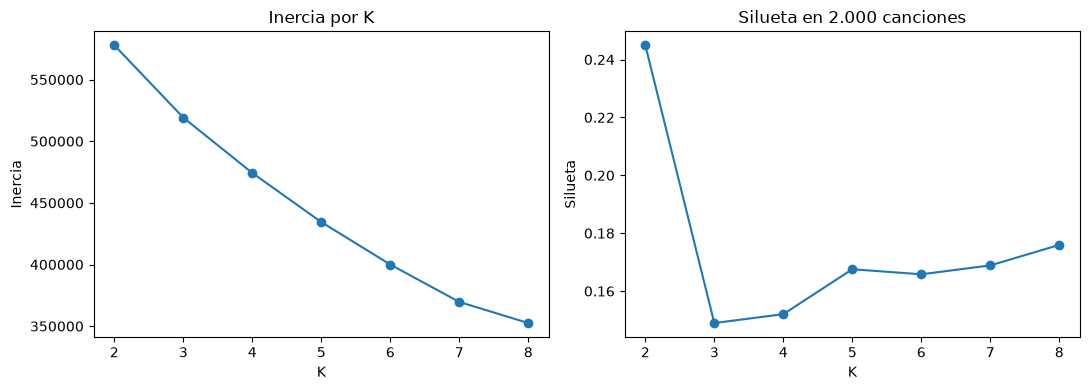
\includegraphics[width=0.87\linewidth]{04a_lucas_k_selection.png}
\caption{Inercia y silueta para $K=2,\ldots,8$. La curva apoya una solución descriptiva de dos grupos; la silueta máxima usada es 0,245. Figura extraída de la salida ejecutada del notebook 04a.}
\label{fig:k-selection}
\end{figure}

Se eligió $K=2$ por el balance entre lectura e indicador, con silueta 0,245.
Este valor indica separación limitada, no dos clases naturales de canciones.
Los perfiles se describieron con estadísticas en unidades originales y la
popularidad se consultó \emph{después} de agrupar, únicamente como descriptor.

\begin{table}[htbp]
\centering\small
\begin{tabular}{lrrrrrr}
\toprule
Grupo & Canciones & Energía & Acústica & Loudness & Bailabilidad & Popularidad mediana \\
\midrule
0 & 54.011 & 0,762 & 0,078 & $-6,140$ & 0,607 & 34 \\
1 & 17.781 & 0,295 & 0,828 & $-13,033$ & 0,468 & 29 \\
\bottomrule
\end{tabular}
\caption{Perfil del entrenamiento. Los valores acústicos son medianas descriptivas en escala original. La popularidad no intervino en K-Means.}
\label{tab:clusters}
\end{table}

El grupo 0 reúne principalmente canciones más enérgicas, menos acústicas y
con mayor \code{loudness}; el grupo 1, canciones más acústicas y suaves. La
mediana de popularidad difiere cinco puntos, sin que esta comparación pruebe que
pertenecer a un grupo cause mayor popularidad. PCA se utilizó solo para proyectar
la matriz estandarizada en dos ejes: ambos explican conjuntamente 44,1\,\% de
la varianza, por lo que la figura omite más de la mitad de la información.

\begin{figure}[htbp]
\centering
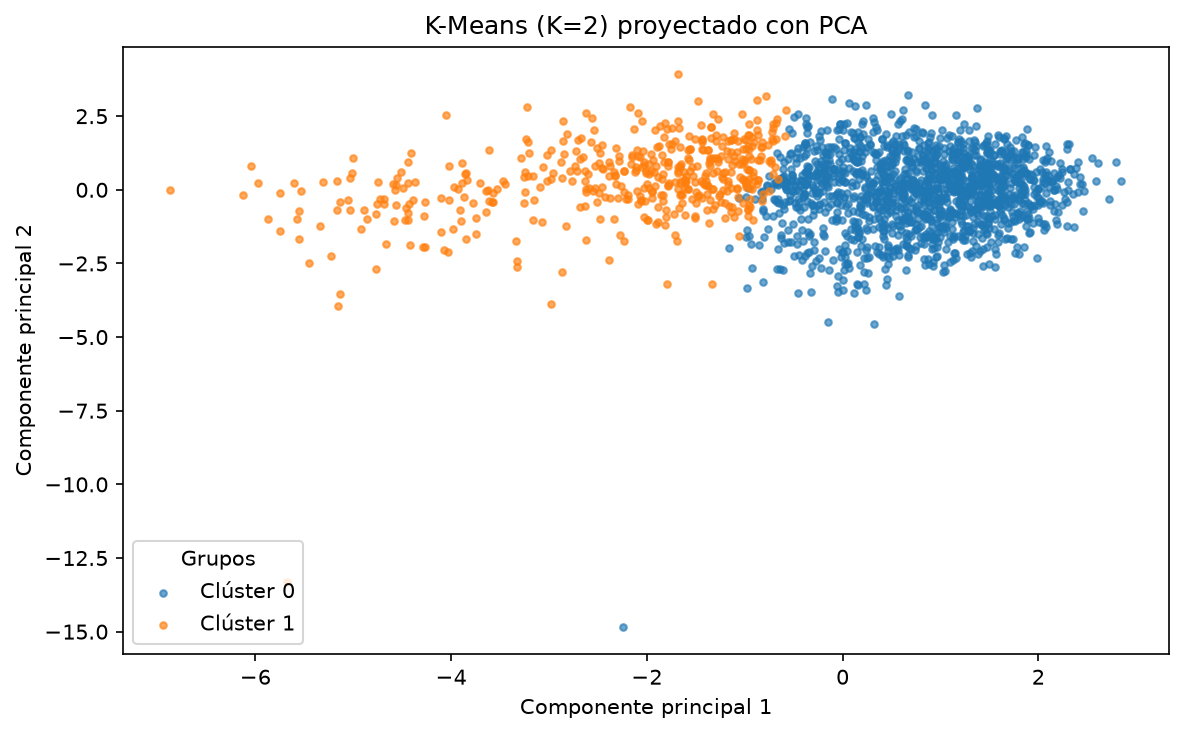
\includegraphics[width=0.82\linewidth]{04a_lucas_clusters_pca.png}
\caption{Proyección PCA de los dos grupos de K-Means. El solapamiento visible concuerda con la silueta moderada; la proyección no es evidencia de separación perfecta en diez dimensiones.}
\label{fig:clusters-pca}
\end{figure}

\subsection{Estabilidad de los perfiles}

Se repitió $K=2$ con el mismo entrenamiento y la misma semilla bajo dos cambios
aislados: transformar \code{duration_ms} con $\log(1+x)$ antes de escalar, y
retirar \code{loudness}. Los números de grupo son arbitrarios; la concordancia
se calculó después de alinear las etiquetas. ARI compara particiones sin
depender de esos nombres.

\begin{table}[htbp]
\centering\small
\begin{tabular}{lrrrr}
\toprule
Configuración & Silueta & ARI vs. base & Coincidencia & Tamaños \\
\midrule
Base, diez atributos & 0,245 & 1,000 & 100,000\,\% & 54.011 / 17.781 \\
Duración $\log(1+x)$ & 0,241 & 0,968 & 99,258\,\% & 53.954 / 17.838 \\
Sin \code{loudness} & 0,209 & 0,807 & 95,194\,\% & 51.769 / 20.023 \\
\bottomrule
\end{tabular}
\caption{Sensibilidad de la partición K-Means. ARI y coincidencia se comparan con la solución base sobre las mismas canciones.}
\label{tab:cluster-sensitivity}
\end{table}

Los dos perfiles siguen siendo reconocibles en ambas variantes. Retirar
\code{loudness} reduce la silueta y mueve más observaciones, señal de que esa
variable contribuye a la separación. Los resultados no validan estabilidad
frente a otras muestras, elecciones de $K$ o métodos de agrupamiento.

\section{Conclusiones y uso compartido}

Ridge completo es la mejor de las variantes supervisadas evaluadas para el
MAE de esta prueba aleatoria. La mejora depende marcadamente de géneros y
persiste, con límites, cuando se apartan artistas principales. La regresión
subestima sistemáticamente las canciones con popularidad al menos 70; por ello
el ranking sirve como filtro exploratorio retrospectivo, no como sustituto del
criterio humano. K-Means aporta un lenguaje descriptivo para explorar familias
acústicas, pero sus grupos no son categorías rígidas ni predicen por sí mismos
la popularidad.

Para el notebook integrador queda por medir si el ranking del 10\,\% cubre de
forma distinta los dos perfiles K-Means. \emph{Esta auditoría es una hipótesis,
no un resultado}.

\subsection{Traspaso a Ignacio y César}

Como trabajo posterior, una evaluación temporal requeriría fechas válidas;
extrapolar a Spotify exige una muestra con frecuencias naturales de géneros.

\begin{enumerate}
\item Reproducir el notebook 04a siguiendo \path{docs/ea2/lucas.md}; verificar
la huella de la fuente, los 89.740 \code{track_id} únicos y la huella de la
prueba común antes de comparar resultados.
\item Reutilizar las funciones del protocolo compartido y reservar la misma
prueba aleatoria. Seleccionar hiperparámetros en validación propia; el
diagnóstico agrupado exige una selección nueva dentro de esa partición.
\item Llevar al notebook 05 los resultados de las Tablas~\ref{tab:random-test},
\ref{tab:artist-test}, \ref{tab:kpi} y \ref{tab:cluster-sensitivity}, con sus
soportes y límites. Contrastar allí los enfoques de los tres integrantes antes
de redactar una conclusión de equipo.
\item En la revisión cruzada, explicar por qué la señal de género puede estar
amplificada por el muestreo, qué significa que todos los populares de prueba
reciban predicción inferior a 70, cómo se calculó el lift y por qué la silueta
0,245 obliga a una interpretación prudente de los grupos.
\end{enumerate}

Las figuras de modelamiento y clustering proceden del notebook 04a; las dos
figuras de contexto proceden del EDA de EP1. El archivo principal de este
informe es \path{docs/ea2/informe_lucas/main.tex} y el PDF compilado queda en
esa misma carpeta. El código, notebook, imágenes y documento son archivos
locales de la rama \code{feature/ea2-modeling-lucas} hasta que el equipo los
integre. Así, la revisión puede hacerse sobre evidencia trazable sin confundir
el informe individual con la entrega conjunta.
